\chapter{The Quest for Meaning in Video}
\label{ch:quest}

\section{Introduction} % (fold)
\label{sec:introduction}

% start intro: consider example of a video segment; indicate how its easy for humans to `understand' the content on multiple levels
Interpreting moving images is not a hard task. The medium film is often described as `dictatorial' because of the way the audience is immersed in a multi-modal experience controlled by the content's creators. When watching a film, we sit back and relax, passively taking in the presented information without much effort. A similar ease is reflected in our use of the word `couch potato' to describe the passive role of television audiences. Watching film or video gives us almost immediate access to a wide range of information about what is presented on screen. We recognise objects on screen and understand words that spoken in a language we know. We are also quick to infer a larger picture around the things we perceive, like personality traits of characters on screen and our emotional stance towards them. While most of these things happen extremely quickly and seemingly automatically to us humans, computers often have a hard time even starting to perceive a visual representation of an object.

% explain how computers are having difficulties. in recognition, spatio/temporal segmentation (figure ground), qualitative evaluations are even more difficult.
When we attend to visual content depicting parts of the world around us, we can't help ourselves from seeing its parts as separate entities. We recognise objects as if they stand out from their background even though they are simply patterns of colours on a two dimensional surface. To a computer, tasks like object segmentation and recognition are hard because visual information needs to be interpreted in some form of sequential processing. Digitally, images are usually represented by collections of numbers indicating local intensities (e.g. brightness) at the different points that make up the image. How to calculate from this information, which objects are present, and what other concepts can be assigned to an image is studied in the field of computer vision. Although recent years have seen important advances in the use of high-level semantical concepts in tasks like video concept detection and concept-based video retrieval \cite{Snoek:2009dq, Snoek:jf, Worring:2007vm, Chang:2008wh}, computational methods commonly have difficulties in performing both reliably and generally.

% setup chapter
% scope of this chapter
Because of the often elusive character of concepts like meaning and understanding, we take care to keep goals for this chapter humble. The intension is not to give an accurate explanation of daunting concepts like meaning or semantics, nor is it to give an accurate account of the diverse work on signifying systems such as in the field of semiotics. This first chapter is meant to briefly introduce the difficulties that current computational methods have in arriving at meaningful interpretations of visual content. To this purpose we formulate a framework of computational analyses of meaning that serves to establish terminology to work with in this work, rather than to make claims about the deeper functioning of human understanding or signifying systems. The next section addresses two high-level challenges to the goal of finding meaning in video and indicates how they arise. Of these, the \emph{semantic gap} is the most poignant and we take a look at how computational approaches aim to overcome this problem.

% section introduction (end)

\section{Challenges in Computational Interpretation of Visual Content}

% from world -> representation -> concepts
As video content possesses most of its information in the visual stream, most research into the interpretation of video has focussed on the analysis of visual content \cite[ch.~2]{Snoek:2009dq}. To better understand what is going on in the interpretation of visual content by both humans and computers, it helps to model the process from start to end. Figure \ref{fig:understanding_visuals} shows in a high-level model how objects in the world are sensed and consequently rendered in a visual representation. We can think of this process taking place when we photograph a car and end up with a picture of that car as a result. When the representation of an object is next interpreted by someone, we can think of this person as establishing semantical concepts relating to aspects of the depiction. A situation to which we can map this part of the model would be someone looking at the picture and recognising the car.

\begin{figure}[htbp]
  \centering
    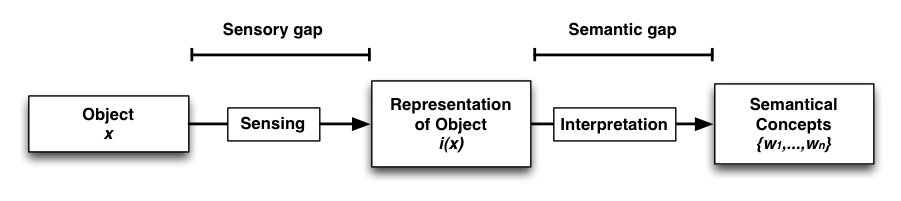
\includegraphics[width=.8\textwidth]{img/understanding_visuals}
  \caption{A high level model of the interpretation of visual media content}
  \label{fig:understanding_visuals}
\end{figure}

% first problem: sensory gap
A first source of complication in the process from object to its interpretation, is the \emph{sensory gap}, described by Smeulders et al. as follows:

\begin{quote}
  ``The sensory gap is the gap between the object in the world and the information in a (computational) description derived from a recording of that scene.''\cite{Smeulders:2000tx}
\end{quote}

% sensory gap explained
The sensory gap makes accurate description of objects in the world difficult as it introduces uncertainty about what aspects of the object are represented. Characteristics of illumination, occlusion, clutter and camera viewpoint all affect the representation of a sensed object. When detailed knowledge about the recording conditions is absent, it is impossible to know which parts of the sensory information should be attributed to the state of the object and which are due to incidental artefacts. Different 3D objects can yield the same 2D representation and differently coloured objects might be represented by identical colour values. This also works the other way, as one object may appear very different in shape and colour on different images depending on illumination and camera viewpoint.

% second problem: semantic gap
A second issue that challenges meaningful interpretation of visual content is the \emph{semantic gap} that lies between a digital representation and the conceptual interpretation we address to it. Snoek and Worring adapt the original definition from \cite{Smeulders:2000tx} to specifically fit the medium video when they describe the semantic gap as:

\begin{quote}
  ``The lack of correspondence between the low-level features that machines extract from video and the high-level conceptual interpretations a human gives to the data in a given situation.''
\end{quote}

One of the causes of the semantic gap is that the way people perceive images is mostly contextual\cite{Smeulders:2000tx}. We look for concepts that are already familiar from our environment or earlier encounters with visual content. Our perception of a simple object is determined by our vast background of personal experience and cultural upbringing. In contrast to these contextual interpretations, computational image descriptions rely purely on data-driven features that can be extracted from the content. Difficulties arise when there is a mismatch between the two.

% subjective interpretations; feeling and emotions
Another cause of the gap are interpretations that are subjective in nature. Semantical concepts relating to feelings and emotions can vary widely across different people. Deciding computationally whether concepts such as ``romantic'' or ``funny'' apply to a piece of content is hard when there is no agreement about the interpretation to begin with.

% concepts combined into larger meanings
Perceived concepts are also combined to infer a larger story around the things we actually see. These knowledge-based interpretations enable us to perceive deeper layers of meaning that are not in itself explicitly represented. An important example of this is the way `readers' of narrative texts or moving images combine elements in their aim for \emph{coherence}\cite[p.~38]{Bordwell:1985tz} \cite{gernsbacher1995coherence, Graesser:1994va}. High-level concepts like coherence over time are usually not explicitly represented in digital content and can be hard to compute algorithmically.

% large variety in appearance of visual concepts 
Even if there is little context dependency in the perception or recognition of an object in video, it might still be hard for computational methods to produce appropriate semantical labels. This is due to the wide variety in appearance of visual concepts. Determining whether a clock is present in a video can be difficult because of the many different sizes, shapes and colours clock can have. 

All of these issues contribute to the gap between the low level features extracted from video and the interpretations we humans give to them. Challenges posed by the semantic gap are of mayor concern to the research community focussing on multimedia retrieval based on querying by user defined semantical concepts. It is thus relevant to different scientific disciplines such as computer vision, information retrieval, machine learning and human-computer interaction. In the next section briefly reviews computational strategies that aim to narrow the semantic gap.

\section{Computational Undertakings of the Quest for Meaning}

Although video content has a multi-modal nature, that may consist of sounds, spoken language, a recorded visual stream, animations and textual information in (sub)titles, it's defining characteristic is the presence of a sequence of images. While some works investigate the role of auditory\cite{Wang:2000vf} and textual features\cite{Kuwano:2000wy} in video analysis, most efforts to narrow the semantic gap in video systems focus on the visual modality and try to make use of the features that can be extracted from it. This section gives a brief overview of the strategies to narrow the semantic gap in that is apparent in the computational interpretation of video content.

\subsection{Feature Extraction}
[Video structuring, indexing and retrieval based on global motion wavelet coefficients]\cite{Bruno:2002tt}

\subsubsection{Visual Features}

In their broad overview of concept-based video retrieval techniques, Snoek and Worring point to the following categories of visual features that are commonly used in video analysis.

\begin{itemize}
  \item \textbf{Colour} - Colour provides rich features as it is very good at characterising the appearance of objects. Different colour spaces can be used to represent the values pixels of an image take along the continuous colour spectrum.

  \item \textbf{Texture} - 

  \item \textbf{Shape} - 

  \item \textbf{Global} - 

  \item \textbf{Region} - 

  \item \textbf{Keypoints} - 

  \item \textbf{Temporal} -  Besides addressing aspects of single video frames, one can also capture how characteristics of these frames develop over time. By following how frames change over time, patterns of motion can be tracked to describe camera motion, motion of regions or points and even segmented objects.

\end{itemize}


\subsubsection{Structural Features}
[cite bordwell \& Thompson: analysis of context dependency]
% hypervideo as form of 1 narrative 2 navigation, link to database documentary
[HyperCafe: Narrative and Aesthetic Properties of Hypervideo \cite{Sawhney:1996tk}]

Besides 

\subsubsection{Textual features}
`` text search against transcript narrative text provides almost all the retrieval capability, even with visually oriented generic topics.''
[Addressing the Challenge of Visual Information Access from Digital Image and Video Libraries]\cite{Christel:2005td}

\cite{Kuwano:2000wy}

\subsubsection{Audio features}


\subsubsection
Human interaction [Relevance feedback: A power tool for interactive content-based image retrieval]\cite{Rui:1998uj}
[collaborative filtering] \url{http://en.wikipedia.org/wiki/Collaborative_filtering}

\subsection{Supervised Learning}

Once features are extracted for a collection of videos, they can be studied to see how they relate to the concepts that are detected within the videos. The paradigm of supervised learning looks to find the relation between features describing instances of data and classifications that can be attributed to them. The approach in supervised learning is to provide a large set of training examples along with the known classification or labelling of the content. Different methods can be used to determine a function that optimally describes how features are combined into a calculation of the probability that an instance should be labeled with a particular classification.

% TODO formal def


\section{Outstanding Challenges} % (fold)
\label{sec:outstanding_challenges}

% the problem of acquiring labelled data for ML approaches

% wide domains e.g. ugvc

% temporal processing is computationally costly and time consuming

% problem of keeping ML techniques up to date in a dynamical environment where new content is added every minute (and a lot of it as we will see when we discuss user generated online video)

% section outstanding_challenges (end)


\section{Discussion} % (fold)
\label{sec:discussion}

% section discussion (end)




